\chapter{Fundamentos Científicos e Tecnológicos}

% cap 2: fundamentos científicos e tecnológicos
%     (pegue apenas os mais citados, siga a Elaine)
%     2.1. Computação em Nuvem, Fog e Edge
%     2.2. Plataformas de processamento distribuído
%         - arq lambda, kappa, (vide guilherme)
%         - MapReduce, Hadoop, Spark, Storm
%     2.3. Apache Flink
%     2.4. Mineração de Dados
%     2.5. Mineração de Stream
%         - quem são, o que consomem
%         (BigFlow apud \cite{Gaber2005}) Mining data streams: A Review.
%     2.6. Novelty Detection
%     2.7. O algoritmo Minas

\section{Computação em Nuvem, Borda e Névoa}

% Para descrever os modelos de computação em nuvem, borda e névoa, é necessário
% abordar o conceito de distância e densidade em redes. Distância pode ser definida como o número de saltos (\emph{hops}), latência, distância geográfica ou combinação destas.
% Densidade é extraída da distância, projetando a mesma num hiper-espaço de maneira que os
% nós com menor distância entre si fiquem mais próximos. Então quando existe um
% grande número de nós numa mesma região diz-se que ela é densa, quando há poucos
% nós em uma região, esparsa. Acredita-se que data centers, backbones e nuvens publicas
% formem uma concentração de nós e quanto mais próximo do usuários finais (folhas)
% mais esparso é esse hiper-espaço.

% Definir internet e rede (borda, centro, etc)
% Classificando a internet por sua densidade podemos dizer que ao centro estão
% os \emph{data centers} e nuvens públicas em seguida o núcleo interconectando redes diversas,
% redes locais e a Borda composta pelos nós folha dentro de uma rede local.

% O modelo de Computação em Nuvem (\emph{Cloud Computing})
% permite alocar recursos como redes, servidores, armazenamento, aplicações    e serviços
% de maneira conveniente e seu provisionamento ágil concede elasticidade para atender
% demandas variáveis com custo mínimo \cite{NIST2011}.

% Definição de Cloud Computing

\subsection{Computação em Nuvem}

A computação em nuvem (em inglês, \emph{cloud computing}), ou simplesmente nuvem
(\emph{cloud}), habilita o acesso através da rede a um grupo compartilhado de
recursos de computação configuráveis (servidores, redes, aplicativo,
armazenamento, serviços, etc.) que podem ser provisionados ou liberados sob
demanda e rapidamente com o mínimo esforço de gerenciamento ou interação com o
provedor de serviços \cite{NIST2011}. As principais características do
\emph{cloud computing} são:

% Alternativamente, a Computação na Borda (\emph{Edge Computing}) destaca-se no
% processamento em tempo real de dados originários da própria borda além de atender
% preocupações de segurança e privacidade \cite{Shi2016}.

\begin{itemize}
    
    \item \textbf{Serviço sob Demanda:} o cliente pode provisionar ou liberar
    capacidades de computação (ex: tempo de servidor e armazenamento) conforme o
    necessário sem requer interação com o provedor de serviço;
    
    \item \textbf{Amplo acesso à rede:} o acesso aos recursos de computação e
    capacidades ocorre pela rede através de mecanismos padrões que permitem o
    acesso por plataformas heterogêneas (celulares, computadores, tablets, etc.)
      
    \item \textbf{Agrupamento de recursos:} para servir múltiplos clientes, os
    recursos de computação são agrupados usando o modelo \emph{multi-tenancy}
    com recursos físicos e virtuais diferentes dinamicamente atribuídos e
    reatribuídos de acordo com a demanda do cliente;
    
    \item \textbf{Elasticidade:} as capacidades de computação são rapidamente
    provisionadas ou liberadas, em alguns casos automaticamente, para escalar
    conforme a demanda;
    
    \item \textbf{Serviço mensurado:} os recursos de computação são monitorados,
    controlados e reportados fornecendo transparência para o provedor de
    serviços e para o cliente sobre as capacidades que foram consumidas.

\end{itemize}

Segundo, \citeonline{NIST2011}, a implantação da Computação em Nuvem pode
ocorrer através dos seguintes modelos:

\begin{itemize}
    
    \item \textbf{Nuvem privada:} a infraestrutura da nuvem é provisionada e
    dedicada para um único cliente ou organização. Nesse modelo, o cliente
    gerencia e controla a infraestrutura, ou pode delegar essas tarefas a uma
    empresa terceira. A infraestrutura pode estar dentro ou fora das instalações
    da organização proprietária;

    \item \textbf{Nuvem comunitária:} a infraestrutura de nuvem é fornecida para
    um grupo exclusivo de clientes que compartilham de um mesmo interesse
    (requerimentos de segurança, desempenho, políticas, etc.). Esse tipo de
    nuvem pode ser gerenciado pelo próprio grupo, ou organizações terceiras,
    podendo estar dentro ou fora das instalações da empresa proprietária;

    \item \textbf{Nuvem pública:} a infraestrutura da nuvem é provisionada e
    oferecida para uso público. É gerenciado e operado por um provedor de nuvem.
    
    \item \textbf{Nuvem híbrida:} a infraestrutura desse tipo de nuvem é uma
    composição de duas ou mais modelos de implantação de \emph{cloud} (privada,
    pública e comunitária) que formam um entidade única e são unidos por
    tecnologias padronizadas que habilitam a portabilidade de dados e
    aplicações.

\end{itemize}

% Definição de Computação de Borda 
\subsection{Computação de Borda}

A computação de borda (em inglês, \emph{edge computing}) refere-se às
tecnologias que permitem que a computação seja executada na borda da rede.
Define-se borda ou \emph{edge} como qualquer recurso de computação e de rede ao
longo do caminho entre as fontes de dados e os data centers da nuvem
\cite{Shi2016}. Na borda, é possível fazer armazenamento, processamento e
descarregamento de dados, assim como distribuir as requisições e entregar os
serviços das nuvens aos usuários. \citeonline{Shi2016} ressalta que essas
capacidades dentre outras dos nós da borda (\emph{edge nodes}) possibilita que a
computação de borda reduza a latência na resposta da nuvem pré-processando os
dados nos nós da borda, aproveitando melhor a banda e a transmissão de dados, e
também consumindo menos recursos de computação na nuvem. Além disso, o autor
ainda acrescentar que o \emph{edge computing} pode aumentar a privacidade dos
dados uma vez que o dado pode ser processado no próprio dispositivo final.

A computação de borda tenta trazer a computação mais próxima das fontes de
dados, como mostra a Figura \ref{edge-computing}. Como é observado na figura, os
componentes desse tipo de computação podem ser tanto produtores como
consumidores, não só requisitando serviços e conteúdo da nuvem, mas também
realizando tarefas da nuvem. Algumas aplicações da computação de borda são: nós
de borda fazendo análise de vídeo; diminuir a latência da nuvem para sistemas
críticos; descarregar a nuvem de parte da computação, pois a borda também tem
capacidade de processamento; privacidade dos dados produzidos por \emph{smart
homes} e sensores IoT, pois dados sensíveis não precisam ir para a nuvem,
liberando também cargas de dados na rede; processamento distribuído nos nós da
borda de dados provenientes de milhões de sensores em cidades inteligentes.


\begin{figure}[ht]
\centering
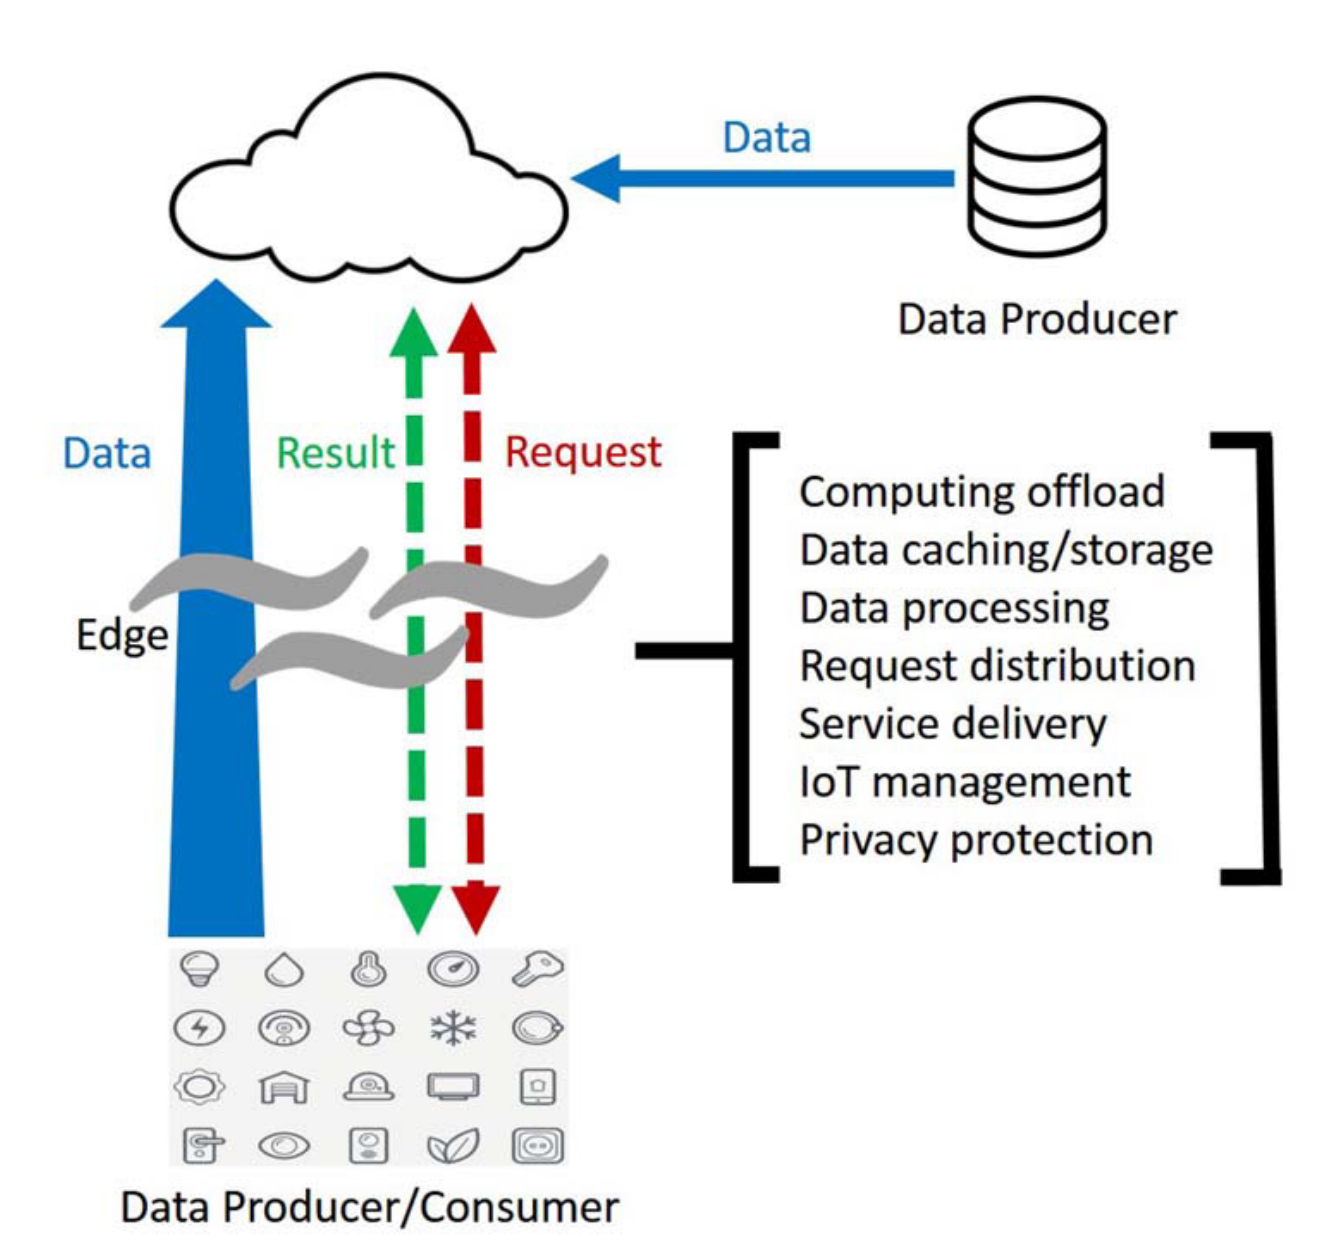
\includegraphics[width=0.6\textwidth]{figuras/edge-computing.png}
\caption{Paradigma de \emph{Edge Computing} \cite{Shi2016}.}
\label{edge-computing}
\end{figure}

\subsection{Computação em Névoa}

\citeonline{Dastjerdi2016} e \citeonline{IEEECommunicationsSociety2018}
mencionam que a enorme massa de dados gerados por ambientes IoT pode ser
processada pela nuvem, entretanto a latência produzida pela transferência desses
dados para a nuvem e o retorno do resultado não são tolerados por sistemas
críticos que sejam sensíveis a latência (monitoramento de saúde e resposta a
emergências). O autor ainda acrescenta que enviar tantos dados a \emph{cloud}
para processamento e armazenamento pode ser ineficiente e não escalável devido a
saturação de dados na rede. O \emph{edge computing} foi proposto para trazer o
processamento e armazenamento para os dispositivos de borda tentando solucionar
esses problemas, porém os dispositivos de borda não podem lidar com várias
aplicações IoT competindo pelos seus recursos limitados, o que poderia causar a
contenção dos recursos e aumento na latência do processamento
\cite{Dastjerdi2016}. Portanto, para solucionar estas questões de latência e
capacidade limita dos dispositivos de borda, a computação em névoa foi proposta.

A computação em névoa (em inglês, \emph{fog computing}) é um paradigma que traz
as capacidades de computação, armazenamento e rede para próximo das fontes dados
e dos dispositivos finais, mas não necessariamente localizados na borda
\cite{Bonomi2012} \cite{Dastjerdi2016} \cite{IEEECommunicationsSociety2018}.
Esse tipo de computação evita a contenção dos recursos dos dispositivos mais
próximos às fontes de dados fornecendo-os capacidade de nuvem e coordenando-os
geograficamente distribuídos. \citeonline{Bonomi2012} e
\citeonline{Dastjerdi2016} veem o \emph{fog computing} como complementar da
\emph{edge computing}, podendo a computação em névoa aproveitar os recursos da
nuvem e da borda. \citeonline{IEEECommunicationsSociety2018} considera que a
principal diferença entre esses dois tipos de computação está no número de
camadas. Enquanto o \emph{edge computing} tem camadas menores, pois atua só nos
dispositivos de borda, o \emph{fog computing} tem mais camadas e um modelo
hierárquico, pois não atua só na camada de borda.

Segundo \citeonline{Bonomi2012} e \citeonline{Dastjerdi2016}, as principais
características da computação em névoa são:

\begin{itemize}

    \item \textbf{Mobilidade:} é essencial que as aplicações \emph{fog} sejam
    capazes de se comunicar com dispositivos móveis, por exemplo, utilizando
    protocolos que considerem a mobilidade dos nós;

    \item \textbf{Heterogeneidade:} os nós nesse tipo de paradigma possuem
    configurações e formatos diferentes e podem estar implantados em ambientes
    distintos;

    \item \textbf{Baixa Latência:} a computação em névoa foi proposta para
    atender aplicações que requeiram baixa latência (monitoramento de saúde,
    jogos, realidade aumentada, etc.);

    \item \textbf{Distribuição geográfica:} o \emph{fog computing} possui
    milhares de sensores e dispositivos distribuídos geograficamente e a
    consciência da localização deles (em inglês, \emph{location awareness});

    \item \textbf{Alto número de nós:} seguindo os ambientes IoT, a computação
    em névoa pode ser composta por milhares de nós;

    \item \textbf{Interoperabilidade e federação:} os componentes da computação
    em névoa devem ser capazes de interoperar, e o serviços devem ser federados
    ao longo de diferentes domínios;

    \item \textbf{Uso de fluxo de dados e aplicações em tempo real:} a
    computação em névoa pode envolver aplicações que processam em lote, mas na
    maior parte das vezes envolve aplicações com requisito de processamento em
    tempo real, e para isso fazem o uso de fluxo de dados. Por exemplo, os
    sensores de um rede IoT inscrevem a informação no fluxo de dados, a
    informação é processada, e os \emph{insights} extraídos são traduzidos em
    ações nos componentes atuadores.

\end{itemize}

Algumas aplicações para computação em névoa são: cidades inteligentes e
semáforos inteligentes que enviam sinais de alerta aos veículos e coordenam os
sinais verdes com outros semáforos através de sensores (veículos, pedestres,
ciclistas); na área de saúde para monitorar e prever situações de pacientes que
estão conectados a sensores; em prédios inteligentes que são dotados de sensores
de umidade, temperatura, qualidade do ar, ocupação, então a partir das
informações deles é possível alertar os ocupantes do prédio em algum caso de
emergência.

% \emph{Edge} é por vezes chamado de Computação em Névoa (\emph{Fog Computing})
% contudo \citeonline{IEEECommunicationsSociety2018} indica diferenças como exclusão do
% modelo \emph{cloud} e limitação a poucas camadas (por exemplo, somente os nós folha de uma rede)
% no modelo \emph{edge} em direto contraste com a inclusão de \emph{cloud} e hierarquias
% maiores. \emph{Fog} também atende gerenciamento da rede, armazenamento e controle.

% Fog works with the cloud, whereas edge is defined by the exclusion of cloud. Fog
% is hierarchical, where edge tends to be limited to a small number of layers. In
% additional to computation, fog also addresses networking, storage, control and
% acceleration. \cite{IEEECommunicationsSociety2018}

% Definição de Fog Computing
% o que é e como se relaciona com IoT e se diferencia das outras

% From our point of view, edge computing is interchangeable with fog computing [19], 
% but edge computing focus more toward the things side, while fog computing focus more 
% on the infrastructures ide.

% Esse modelo de computação distribuída desde os nós folha até o centro é motivado
% pela mudança do \emph{statu quo} do fluxo dos dados na internet: tradicionalmente
% os dados são produzidos pelos dispositivos de borda imediatamente enviados à 
% \emph{cloud} (produção, \emph{upstream}),
% que armazena e processa recursos derivados servido-os através de requisição-resposta
% (consumo, \emph{downstream}) a mais clientes.
% Com a ampliação da Internet das Coisas (\emph{Internet of Things}, IoT) e consequente
% ampliação sem precedentes do volume de dados gerados, mudando o relação de consumo
% e produção \cite{Shi2016}, arquiteturas tradicionais como \emph{cloud} podem não
% ser capazes de lidar com esses dados por falta de banda o que leva as
% propostas de distribuição vertical do processamento em \emph{fog} \cite{Bonomi2012, Dastjerdi2016}.

% Previous work such as micro datacenter [12], [13], cloudlet [14], and fog computing [15]
% [15] F. Bonomi, R. Milito, J. Zhu, and S. Addepalli,
% “Fog computing and its role in the Internet of things,” 
% in Proc. 1st Edition MCC Workshop Mobile Cloud Comput., Helsinki, Finland, 2012, pp. 13–16.

% Fog Computing: Helping the Internet of Things Realize Its Potential
% \cite{Dastjerdi2016}
% The Internet of Things (IoT) could enable
% innovations that enhance the quality of life, but it
% generates unprecedented amounts of data that
% precedented amounts of data that can be useful in many ways, par-
% are difficult for traditional systems, the cloud, and
% even edge computing to handle. Fog computing
% is designed to overcome these limitations.

\section{Mineração de Dados e Fluxo de Dados}

% Faria nem Silva definem ou citam data mining
% A data stream (DS) is a sequence of examples that arrive continuously. They are
% continuous, unbounded, flow at high speed and have a data distribution that
% may change over time \cite{Silva2013}. In DS scenarios, new concepts may
% appear and known concepts may disappear or evolve. \cite{Faria2016nd}

A Mineração de Dados é o processo de descoberta de padrões em conjuntos de dados
utilizando métodos derivados de aprendizagem de máquina, estatística e banco de
dados \cite{Gaber2005}. Um caso de mineração de dados é \emph{Big Data} onde o
conjunto de dados não pode ser processado em um tempo viável devido a limitações
como armazenado na memória ou armazenamento principal.

% Data stream mining is concerned with the extraction of knowledge from large
% amounts of continuously generated data in a non-stationary environment. Novelty
% detection (ND), the ability to identify new or unknown situations not
% experienced before, is an important task for learning systems, especially when
% data are acquired incrementally (Perner 2008). In data streams (DSs), where new
% concept can appear, disappear or evolve over time, this is an important issue to
% be addressed. ND in DSs makes it possible to recognize the novel concepts, which
% may indicate the appearance of a new concept, a change in known concepts or the
% presence of noise (Gama 2010).
% 
% Perner P (2008) Concepts for novelty detection and handling based on a case-based
% reasoning process scheme. Eng Appl Artif Intell 22:86–91
% 
% Gama J (2010) Knowledge discovery from data streams, vol 1, 1st edn. CRC press chapman hall, Atlanta

% dados massivamente e continuamente gerados e não persistentes. Fp

% \cite{Gaber2005} Cited by 1174
% Data mining is that interdisciplinary field of study that can extract models
% and patterns from large amounts of information stored in data repositories
% [30, 31, 34].
% 
% Recently, the data generation rates in some data sources become faster than ever
% before. This rapid generation of continuous streams of information has
% challenged our storage, computation and communication capabilities in computing
% systems. Systems, models and techniques have been proposed and developed over
% the past few years to address these challenges [5, 44]

Além da dimensão de armazenamento outra dimensão que afeta a maneira como dados
são modelados e manipulados é o tempo. Um Fluxo de Dados (\emph{Data Stream}) é
uma sequência de registros produzidos a uma taxa muito alta, associadas ao tempo
real, ilimitados, que excede recursos de armazenamento e comunicação \cite{Gaber2005}.
Modelos de mineração de fluxo de dados atendem a esses desafios utilizando
restrições como apenas uma leitura do conjunto de dados e complexidade
de processamento menor que linear \cite{Gama2007, Gaber2005}.

% A data stream is a sequence of unbounded, real-time data records that are
% characterized by the very high data rate, which stresses our computational
% resources, and can be read only once by processing applications [13,8,1,9]
 
% [1] B. Babcock, S. Babu, M. Datar, R. Motwani, J. Widom, Models and issues in
% data stream systems. In: Proceedings of Principles of Database Systems
% (PODS’02), pp. 1–16, 2002. \cite{Babcock2002}

% [2] G. Boone, Reality mining: browsing reality with sensor networks.
% In: Sensors Online, vol. 21, 2004.

% [3] V. Cantoni, L. Lombardi, P. Lombardi, Challenges for data mining in
% distributed sensor networks. ICPR (1) 1000–1007, 2006

% [8] M.M. Gaber, A. Zaslavsky, S. Krishnaswamy, Mining data streams: a review.
% ACMSIGMOD Record, 34(2):18–26, 2005.
% 
% [9] M. Garofalakis, J. Gehrke, R. Rastogi, Querying and mining data streams:
% you only get one look a tutorial. In: Proceedings of the 2002 ACM SIGMOD
% International Conference on Management of Data, June 03–06, Madison, Wisconsin,
% 2002.
% 
% [13] S. Muthukrishnan, Data streams: algorithms and applications. In:
% Proceedings of the Four- teenth Annual ACM-SIAM Symposium on Discrete
% Algorithms, 2003.

% Mineração de Fluxo de Dados é análogo à mineração de
% dados e \emph{big data} com a restrição temporal onde um registro é unicamente 
% associado um tempo, dessa forma além de não ser possível manipular o conjunto
% de dados em memória, não é possível recuperar dados fora do intervalo de tempo associado
% a eles.

% ----- wikipedia ------
% 
% Data mining is the process of discovering patterns in large data sets involving
% methods at the intersection of machine learning, statistics, and database
% systems.[1] Data mining is an interdisciplinary subfield of computer science and
% statistics with an overall goal to extract information (with intelligent
% methods) from a data set and transform the information into a comprehensible
% structure for further use.[1][2][3][4] Data mining is the analysis step of the
% "knowledge discovery in databases" process or KDD.[5] Aside from the raw
% analysis step, it also involves database and data management aspects, data
% pre-processing, model and inference considerations, interestingness metrics,
% complexity considerations, post-processing of discovered structures,
% visualization, and online updating.[1]
% 
% [1] "Data Mining Curriculum". ACM SIGKDD. 2006-04-30. Retrieved 2014-01-27.
% [2] Clifton, Christopher (2010). "Encyclopædia Britannica: Definition of Data Mining". Retrieved 2010-12-09.
% [3] Hastie, Trevor; Tibshirani, Robert; Friedman, Jerome (2009).
% "The Elements of Statistical Learning: Data Mining, Inference, and Prediction".
% Archived from the original on 2009-11-10. Retrieved 2012-08-07.
% [4] Han, Kamber, Pei, Jaiwei, Micheline, Jian (June 9, 2011).
% Data Mining: Concepts and Techniques (3rd ed.). Morgan Kaufmann. ISBN 978-0-12-381479-1.
% [5] Fayyad, Usama; Piatetsky-Shapiro, Gregory; Smyth, Padhraic (1996).
% "From Data Mining to Knowledge Discovery in Databases" (PDF). Retrieved 17 December 2008.

% - quem são, o que consomem
% (\citeonline{Viegas2019} \emph{apud} \citeonline{Gaber2005}) Mining data streams: A Review.

\section{Arquiteturas e Plataformas de Processamento de Fluxos}

% - arq lambda, kappa, (vide guilherme)

% Existem diversas maneiras de organizar o caminho das informações em um
% aplicativo de processamento de fluxo de dados. Algumas propostas sao amplamente
% conhecidas como as arquiteturas Lambda (MARZ; WARREN, 2015) e Kappa (KREPS,
% 2014), as quais s˜ao genéricas e focadas no processamento de fluxo.

% A arquitetura Lambda (MARZ; WARREN, 2015) mescla o processamento do fluxos de
% dados com o processamento em lotes. O objetivo dessa mistura é obter, ao mesmo
% tempo, a capacidade de fazer análises em tempo real, e, ao mesmo tempo,
% fazê-las com maior qualidade. Seu processamento é dividido em duas camadas,
% uma camada de processamento online que fornece resultados aproximados com baixa
% latência e uma camada de processamento offline que usa os dados históricos
% disponíveis e fornece resultados mais precisos, embora com maior sobrecarga e
% latência. Além das duas camadas de processamento, a Arquitetura Lambda possui
% uma camada de serviço, que combina dados de ambas as camadas de processamento e
% apresenta ao usuário.

% A arquitetura Kappa, por outro lado, possui apenas as camadas de processamento e
% serviço de fluxo. Seu objetivo é o processamento em tempo real, portanto
% possui a menor quantidade possível de sobrecarga e latência. Sendo assim, é
% natural que esta seja uma arquitetura muito simples e que possua apenas os
% módulos essenciais para um sistema de processamento de fluxo. A arquitetura
% Kappa possui apenas um módulo de processamento on-line que opera através do
% fluxo de dados e fornece informações.

% MARZ, N.; WARREN, J. Big Data: Principles and Best Practices of Scalable
% Realtime Data Systems. 1st. ed. Greenwich, CT, USA: Manning Publications Co.,
% 2015. ISBN 1617290343, 9781617290343. \cite{marz2015big}

% KREPS, J. Questioning the Lambda Architecture. 2014. Disponível em:
% https://www.oreilly.com/ideas/questioning-the-lambda-architecture

Tradicionalmente, aplicações foram construídas com um sistema gerenciador de
banco de dados (SGBD) relacional ou não-relacional associado. Essa arquitetura,
nomeada de arquitetura totalmente incremental por \citeonline{marz2015big},
foi evoluída e simplificada iterativamente durante décadas de uso porém ela não
é adequada para sistemas em tempo real, como os sistema de fluxo de dados.

O volume e velocidade de dados em um \emph{Data Stream} leva a necessidade de
distribuir o processamento acrescentando poder computacional a cada nó
adicionado porém desafios como comunicação eficiente e sincronização de estado
entre os nós assim como tolerância a falhas aumentam a complexidade de
construção de um sistema distribuído em relação a um sistema tradicional. Para
mitigar esses problemas foram propostas arquiteturas de processamento de fluxo
de dados distribuído como arquitetura \emph{lambda} e \emph{kappa} além de
diversas plataformas tanto de \emph{Big Data} com características de tempo real
como especializadas em fluxo de dados.

Arquitetura \emph{lambda} divide o processamento em três camadas: lotes, serviço
e velocidade. A camada de lotes atua sobre o conjunto mestre em modo de leitura
sequencial, armazenando-o em sistema de aquivos distribuído e pré-processando
várias visões sobre esse conjunto mestre, essas visões (armazenadas num SGBD
tradicional) são consumidas pela camada de serviço, que portanto tem acesso
regular (leitura aleatória), no entanto as garantias oferecidas pela camada de
lotes (escalabilidade, consistência, tolerância a falhas) não atendem os requisitos
de latência em um sistema em tempo real, portanto a camada de velocidade
complementa os dados das visões com dados diretamente do conjunto mestre em
tempo real diretamente para a camada de serviço \cite{marz2015big}.

A Figura \ref{lambda} ilustra uma implementação da arquitetura \emph{Lambda}
onde a \emph{Apache Kafka}, \emph{Apache Storm}, \emph{Apache Hadoop}
implementam o conjunto mestre, camada de velocidade e camada de lotes
respectivamente.

\begin{figure}[ht]
\centering
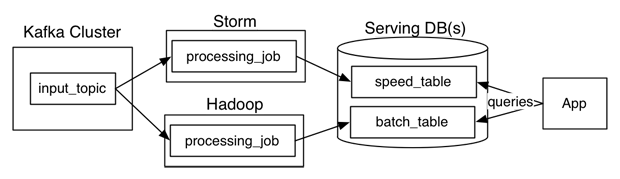
\includegraphics[width=0.6\textwidth]{figuras/lambda.png}
\caption{Arquitetura \emph{Lambda} com detalhes práticos \cite{Kreps2014}.}
\label{lambda}
\end{figure}

No entanto, observações práticas de \citeonline{Kreps2014} mostram que como o
sistema de fila de mensagens (no exemplo \emph{Apache Kafka}) fonte do conjunto
de dados mestre por lidar com diversas fontes, garantir tolerância a falhas,
replicação e armazenamento de longo prazo, poderia ser usado como fonte de
verdade em conjunto com a arquitetura totalmente incremental (tradicional)
substituindo as camadas de lotes e velocidade e o sistema de aquivos distribuído
simplificando a aplicação de três implementações para duas eliminando a
repetição de tarefas executadas pelas camadas de lotes e velocidade que
produziam o mesmo resultado.

Essa arquitetura que limita-se ao processamento de \emph{Stream} apenas
\emph{on-line} destila outras observações quanto a complexidade temporal do
sistema completo de que se uma aplicação não processa os dados em tempo menor
que linear, dados serão perdidos ou a complexidade espacial são será satisfeita,
em resumo, a aplicação sempre deve ser mais rápida que o \emph{Stream}
\cite{marz2015big}.

% - MapReduce, Hadoop, Spark, Storm
% Breve descrição do MapReduce e Hadoop
% O que são e para que servem essas ferramentas

Em sincronia com os desenvolvimentos em arquiteturas de processamento de fluxo,
durante as últimas duas décadas foram construídas diversas plataformas de
processamento para \emph{Big Data} e \emph{Streams}.
% A seguir descrevemos algumas das mais notáveis (?)

\emph{MapReduce} é a primeira plataforma de processamento de conjuntos massivos
de dados que atingiu uso generalizado. Nessa implementação uma biblioteca
gerencia a distribuição, paralelização, tolerância a falhas e balanceamento de
carga e ao usuário resta implementar duas funções: \emph{Map} que recebe uma par
$(chave, valor)$ e emite um conjunto de pares intermediários na mesma estrutura;
\emph{Reduce} recebe uma chave e um conjunto de valores gerado pelo agrupamento
de pares com a mesma chave \cite{Dean2004}.

Em prática um \emph{cluster} tem centenas processadores e o conjunto de dados é
armazenado em um sistema de arquivos distribuído que é lido pela plataforma com
programas escritos por usuários sendo executados sob supervisão de nó mestre.
Essa implementação tem esquema geral de processamento em lotes que não atende o
requisito de baixa latência porém suas vantagens sobrepunham as desvantagens.
\emph{MapReduce} é uma das principais influencias na criação da arquitetura
\emph{lambda} \cite{marz2015big}.

\emph{Apache Hadoop} é uma coleção de ferramentas incluindo: \emph{Hadoop
Distributed File System} (HDFS) um sistema de arquivos distribuído, \emph{Hadoop
YARN} um gerenciador de recursos em cluster e escalonador de trabalhos e,
\emph{Hadoop MapReduce} um sistema baseado em \emph{YARN} implementando o modelo
\emph{MapReduce} \cite{ApacheHadoop2020}.

% Breve descrição do Apache Spark

% Spark is an open-source cluster computing framework with a large global user base.
% It is written in Scala, Java, R, and Python and gives programmers an Application Programming Interface (API)
% built on a fault tolerant, read-only multiset of distributed data items.
% In two years since its initial release (May 2014), it has seen wide acceptability for real-time,
% in-memory, advanced analytics — owing to its speed, ease of use, and the ability to handle
%  sophisticated analytical requirement
% https://dzone.com/articles/streaming-in-spark-flink-and-kafka-1

% Apache Spark is an open-source distributed general-purpose cluster-computing
% framework. Spark provides an interface for programming entire clusters with
% implicit data parallelism and fault tolerance. Originally developed at the
% University of California, Berkeley's AMPLab, the Spark codebase was later
% donated to the Apache Software Foundation, which has maintained it since.

% Apache Spark is a fast and general-purpose cluster computing system. It provides
% high-level APIs in Java, Scala, Python and R, and an optimized engine that
% supports general execution graphs. It also supports a rich set of higher-level
% tools including Spark SQL for SQL and structured data processing, MLlib for
% machine learning, GraphX for graph processing, and Spark Streaming.

\emph{Apache Spark}, analogamente ao \emph{Hadoop}, é um \emph{framework} para
construção de sistemas de computação distribuída em \emph{cluster} com garantias
de tolerância a falhas. No entanto, o modelo de processamento diverge
significativamente do tradicional \emph{MapReduce} utilizando em lugar do HDFS
um multi-set de apenas leitura distribuído (\emph{Resilient Distributed Dataset}
- RDD) com um escalonador de trabalhos representados por grafos acíclicos
direcionados (\emph{directed acyclic graph} - DAG), otimizador de consultas e
motor de execução \cite{ApacheSpark2020}.

% MapReduce programs read input data from disk, map a function across the data,
% reduce the results of the map, and store reduction results on disk.
% Spark's RDDs function as a working set for distributed programs that offers a
% (deliberately) restricted form of distributed shared memory.[8]

Enquanto programas \emph{MapReduce} fazem sua entrada de dados por leitura de um
disco, executam a função \emph{Map} em todos os items, agrupam, executam
\emph{Reduce} e armazenam o resultado em disco novamente, RDD opera com um
conjunto de trabalho distribuído em formato de memória compartilhada com
restrições. Esse conjunto de trabalho distribuído facilita programas iterativos
que são típicos de análise, mineração de dados e aprendizado de máquina.

Foi desenvolvido no AMPLab da Universidade da Califórnia[2] e posteriormente
doado para a Apache Software Foundation[3] que o mantém desde então.

Spark provê uma interface para programação de clusters com paralelismo e
tolerância a falhas.

Apache Spark \ cite{Zaharia} é um 
(execução em computadores não confiáveis) utilizando como premissas: paralelização
e localidade de dados, como 

api em Python (dataframe de pandas)
% ------------------------------------------------------------------------------------------------------


\section{Apache Flink}

Breve descrição do Flink (como esse vai ser usado, precisa explicar um pouco melhor - 2 paginas pelo menos):\\
- arquitetura\\
- modelo de programacao\\
- 1 pequeno exemplo de codigo explicando

\cite{Lopez2018}

% These stream applications are characterized by an unbounded sequence of events, or tuples, that arrive continuously [4]. \cite{Stonebraker2005}

% A number of requirements must be met on distributed stream processing platforms, \citeonline{Stonebraker2005} Stonebraker et al. highlight the most important [4]. 


% the difficulties in anonymizing and extracting knowledge from
% anonymized data, and discuss the main datasets available [6].
% Among the datasets for security research, the most commonly
% used is KDD [10], whose characterization was performed by
% Tavallaee et al. [15]. \cite{Lopez2017}

% \cite{Lopez2017}
% In this paper, we analyze and characterize the traffic of a broadband Internet
% access network by differentiating normal from anomalous traffic, that is marked
% as threat by an IDS. We collected real and anonymized data from a major
% telecommu- nications operator ^1. The dataset is created by capturing 5 TB of
% access data of 373 residential broadband users in the city of Rio de Janeiro,
% Brazil. The dataset contains legitimate traffic, attacks and other security
% threats
% ^1 Anonymized data can be consulted through email contact with authors.

% [4] STONEBRAKER, M., C¸ ETINTEMEL, U., ZDONIK, S. “The 8 requirements of
% real-time stream processing”, ACM SIGMOD Record, v. 34, n. 4, pp. 42–
% 47, 12 2005. ISSN: 01635808. doi: 10.1145/1107499.1107504.
% \cite{Stonebraker2005}
% [80] ANDREONI LOPEZ, M., LOBATO, A. G. P., MATTOS, D. M. F., et al. “Um
% Algoritmo Não Supervisionado e Rápido para Seleção de Caracterı́sticas
% em Classificação de Tráfego”. In: XXXV SBRC’2017, Belém- Pará, PA,,
% 2017.
% [81] ANDREONI LOPEZ, M., LOBATO, A. G. P., DUARTE, O. C. M. B., et al.
% “An evaluation of a virtual network function for real-time threat detection
% using stream processing”. In: IEEE Fourth International Conference on
% Mobile and Secure Services (MobiSecServ), pp. 1–5, 2018. doi: 10.1109/
% MOBISECSERV.2018.8311440.
% [82] CHENG, Z., CAVERLEE, J., LEE, K. “You Are Where You Tweet: A Content-
% based Approach to Geo-locating Twitter Users”. In: Proceedings of the
% 19th ACM International Conference on Information and Knowledge Man-
% agement, CIKM ’10, pp. 759–768. ACM, 2010. ISBN: 978-1-4503-0099-5.
% [83] LOBATO, A. G. P., ANDREONI LOPEZ, M., DUARTE, O. C. M. B. “Um
% Sistema Acurado de Detecção de Ameaças em Tempo Real por Processa-
% mento de Fluxos”. In: SBRC’2016, pp. 572–585, Salvador, Bahia, 2016.


% \{Messa queueing systems - Sistemas de filas de mensagens}
% O que são, para que servem e citar alguns exemplos
% \{Kafka}
% 1 pag

% Apache Flink % Apache Flink is an open-source platform for distributed stream
% and batch data processing. Flink’s core is a streaming data flow engine that
% provides data distribution, communication, and fault tolerance for distributed
% computations over data streams. Flink also builds batch processing on top of the
% streaming engine, overlaying native iteration support, managed memory, and
% program optimization.

% Advantages of Flink:

% Flink streaming processes data streams as true streams, i.e. data elements are
% immediately “pipelined” through a streaming program as soon as they arrive. This
% allows performing flexible window operations on streams.

% Better memory management: Explicit memory management gets rid of the occasional spikes found in Spark framework.

% Speed: It manages faster speeds by allowing iterative processing to take place
% on the same node rather than having the cluster run them independently. Its
% performance can be further tuned by tweaking it to re-process only that part of
% data that has changed rather than the entire set. It offers up to a five-fold
% boost in speed when compared to the standard processing algorithm.

% Apache Spark is considered a replacement for the batch-oriented Hadoop system.
% But it includes a component called Apache Spark Streaming, as well. Contrast
% this with Apache Flink, which is a Big Data processing tool and it is known to
% process big data quickly with low data latency and high fault tolerance on
% distributed systems on a large scale. Its defining feature is its ability to
% process streaming data in real time.

\section{Detecção de Novidade}

Novelty Detection

breve descrição do que sao algoritmos para DN

ver se tem algum survey e citar

\section{O algoritmo MINAS}

Breve descrição do MINAS \cite{Faria2016minas}.

ver paper da profa. Elaine

% discussão de 2020-02-01
Detecção de intrusão em redes
    - riscos de segurança
    % pontos de coleta de dados básicos para a maioria das estruturas de IoT sao Wireless Sensor Networks (WSN) e WSN baseadas em IP,
    % as quais s˜ao vulneráveis e geram uma ameac¸a de seguranc¸a de alto n´ıvel (ADAT; GUPTA, 2018) Adat2018
    % (KASINATHAN et al., 2013), a detecc¸ ˜ao de assinaturas
    % (RAZA; WALLGREN; VOIGT, 2013; SHEIKHAN; BOSTANI, 2016) s˜ao propostos IDSs h´ıbridos com foco 
                % espec´ıfico em ataques de roteamento como sink-hole e redireciona- mento seletivo
    - técnicas de intrusão e tipos de ataques
    - mecanismo de detecção (análise de fluxo de rede -> detecção de anomalia)
    % Guilherme: A tarefa de detecção de intrusão consiste em descobrir, 
    %           determinar e identificar a utilização, duplicação, alteração ou destruição
    %           não autorizada de sistemas de informação (MUKKAMALA; SUNG; ABRAHAM, 2005) Mukkamala2005
    % deteccao por assinaturas (tambem chamada de misuse-detection), deteccao comportamental (tambem chamada de anomaly-detection)e deteccao hıbrida.(MODI et al., 2013).
    % implementacao usualmente é feita por meio de técnicas de AM e MD (BUCZAK; GUVEN, 2016).
    % existem poucos trabalhos [..] online e deteccao de novidade ao problema [..] observado nas surveys (BUCZAK; GUVEN, 2016; MITCHELL; CHEN, 2014; MODI et al., 2013).
    % (FURQUIM et al., 2018), os autores implementam uma arquitetura de 3 camadas (WSN, Fog e Cloud)
    % (MIDI et al., 2017), os autores propuseram um IDS h´ıbrido [...] ativa apenas os módulos [...] especializado em um ataque espec´ıfic
    % (FAISAL et al., 2015)externo ou interno ao Smart Meter.dados do KDD99 [...] precis˜ao, Kappa, consumo de memória, tempo e FAR
    % extensivamente em (Sommer; Paxson, 2010) e (MCHUGH, 2000), é dif´ıcil encontrar boas me- didas de avaliac¸ ˜ao para IDSs
    % (GAMA, 2010) afirma que no contexto de processamento de fluxo, as medidas tradicionais s˜ao impreci- sas.
Detecção de novidades
    % (PERNER, 2007)(GAMA, 2010). A
    - técnicas de Detecção de novidades
    - MINAS (incluir métricas) 
    % (FARIA et al., 2016)
    % ECSMiner (MASUD et al., 2011)
    % AnyNovel (ABDALLAH et al., 2016) s˜ao
    % medidas de Qualidade da Deteccao utilizadas foram Fnew, Mnew, Erro e a quantidade de exemplos rotulados por especialistas que cada técnica requisitou (MASUD et al., 2011)
    - BigFlow (incluir métricas)
Processamento de Streams (big data)
    - cloud?
    % A arquitetura Lambda (MARZ; WARREN, 2015) de duas camadas de CPU (stream e batch) e camada de serviço
    % Kappa (KREPS, 2014) possui apenas um módulo de processamento on-line (apenas as camadas de processamento e servic¸o)
    - redes como stream
    - Atraso
    - Kafka/Spark/Flink
Redes IoT
    - Restrição hardware (Energia, CPU, Mem, Rede)
    - Consideração FOG vs Cloud
%/discussão
